% Kopfzeile beim Kapitelanfang:
\fancypagestyle{plain}{
%Kopfzeile links bzw. innen
\fancyhead[L]{\Large Vorlesung 7 (04.11.2013)}
%Kopfzeile rechts bzw. außen
\fancyhead[R]{}}
%Kopfzeile links bzw. innen
\fancyhead[L]{\Large Vorlesung 7 (04.11.2013)}
%Kopfzeile rechts bzw. außen
\fancyhead[R]{}
% **************************************************
\chapter{Folgen}\label{P5}
\section{Definition: Folgen}\label{5.1}
Sei $X$ eine Menge. Eine \underline{Folge in $X$} ist eine Abbildung $f: \N \to X, x \mapsto f(x) =: a_n \in X$.

\subsection*{Schreibweise}
$(a_n)_{n \in \N} \subseteq X$\\
Varianten: $(a_n)_{n \in \N_0}$, $(a_n)_{n \ge k} = (a_k, a_{k+1}, a_{k+2}, \hdots)$ mit festen $k \in \Z$\nl
Folgen im $\R$ bezeichnet man auch als ``reelle Folgen''

\subsection*{Beispiele}
\en{
\item $a_n = n^2$, $(a_n)_{n \in \N} = (1,4,9,\hdots)$
\item $a_n = (-1)^n$, $(a_n)_{n \ge 0} = (1,-1,1,-1,\hdots)$
\item Konstante Folgen: $a_n = a \forall n \in \N$, $(a_n) = (a,a,a,\hdots)$\\
Dagegen: $\{a_n : n \in \N\} = \{a\}$
}

\section*{Rekursive Definition von Folgen $(a_n)_{n \in \N} \subseteq X$}
\begin{enumerate}[label=(\Roman*)]
\item Angabe von $a_1$
\item Angabe einer Vorschrift, mit der $a_{n+1}$ aus $a_n$ berechnet wird: $a_{n+1} = F(a_n)$ mit einer Funktion $F: X \to X$
\end{enumerate}
Nach Induktionsaxiom ist dann $a_n$ definiert für alle $n \in \N$.

\subsection*{Beispiele}
\en{
\item Potenzen: $a_n = x^n$ ($x \in \R, n \in \N_0$)\\
$a_0 := 1$, $a_{n+1} := x \cdot a_n$
\item Fakultät: $a_n = n!$ ($n \in \N_0$)\\
$a_0 := 1$, $a_{n+1} := (n+1) \cdot a_n$
}

\subsection*{Allgemeiner}
\begin{enumerate}[label=(\Roman*')]
\item Angabe von $a_1 , \hdots , a_k$ ($k \in \N$)
\item $a_{n+1} = F(a_{n-k+1} , \hdots , a_n)$ ($n \ge k$) mit $F: X^k \to X$
\end{enumerate}
Zur Notation: Seien $X_1 , \hdots , X_k$ Mengen.\\
Kartesisches Produkt der $X_1$:\\
$\bigprod_{i=1}^k X_i := X_1 \times \hdots \times X_k := \{\underbrace{(x_1 , \hdots , x_k)}_{k \text{-Tupel (geordnet)}} : x_i \in X_i , 1 \le i \le k \}$\\
$X^k := X \times X \times \hdots \times X$ ($k$ Faktoren)\\
z.B.: $\R^2 = \R \times \R$

\subsection*{Beispiel: Fibonacci-Zahlen}\label{Fibonacci}
$a_0 := 1$, $a_1 := 1$, $a_{n+1} := a_{n-1} + a_n$ ($n \ge 1$)\\
$(a_n) = (1,1,2,3,5,8,13,\hdots)$

\section{Definition: Konvergenz, Grenzwert}\label{5.2}
Eine Folge $(a_n)_{n \in \N} \subseteq \R$ heißt \underline{konvergent}, falls ein $a \in \R$ existiert, so dass gilt:\\
$\forall \eps > 0 \exists n_0 \in \N : |a_n - a| < \eps \forall n \ge n_0$\nl
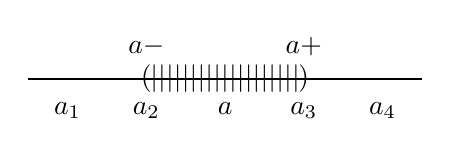
\begin{tikzpicture}[decoration=brace]
\draw(0,0)--(5,0);
\foreach \x/\xtext in {0.5/$a_1$,1.5/$a_2$,2.5/$a$,3.5/$a_3$,4.5/$a_4$}
  \draw(\x,-5pt) node[below] {\xtext};
\foreach \x/\xtext in {1.5/$a-\eps$,3.5/$a+\eps$}
  \draw(\x,+5pt) node[above] {\xtext};
\foreach \x in {1.6,1.7,1.8,1.9,2,2.1,2.2,2.3,2.4,2.5,2.6,2.7,2.8,2.9,3,3.1,3.2,3.3,3.4}
  \draw(\x,0pt) node{$|$};
\draw(1.5,0pt) node{$($};
\draw(3.5,0pt) node{$)$};
\end{tikzpicture}\\
Das heißt: $\forall \eps > 0$ liegen alle bis auf höchstens endlich viele Folgenglieder im Intervall $(a-\eps, a+\eps)$\\
$a$: \underline{Grenzwert (Limes)} der Folge $(a_n)$

\subsection*{Schreibweise}
$\biglim_{n \to \infty} a_n = a$ oder $a_n \to a$ für $n \to \infty$

\subsection*{Beispiel}
Konstante Folge $a_n = a$ (also: $a = a_1 = a_2 = \hdots$) $a_n \to a$

\section{Lemma: Grenzwert von Folgen}\label{5.3}
Jede Folge $(a_n) \subseteq \R$ hat höchstens $1$ Grenzwert.

\subsection*{Beweis}
Sei $a_n \to a$, $a_n \to a'$ und $a \neq a'$.\\
Wähle $\eps := \frac{1}{2} |a-a'| > 0 \Rightarrow \exists n_1 , n_2 \in \N : |a_n - a| < \eps \forall n \ge n_1 , |a_n - a'| < \eps \forall n \ge n_2$\\
Für $n \ge n_0 := max(n_1 , n_2)$ folgt: $|a-a'| \le |a-a_n| + |a_n-a'| < 2 \eps = |a-a'|$ \wspruch

\subsection*{Bezeichnung}
\en{
\item Eine Folge $(a_n)$ mit $a_n \to 0$ heißt \underline{Nullfolge}.
\item Eine Folge, die nicht konvergiert, heißt \underline{divergent}.
}

%\newpage

\section{Beispiele für kon-/divergente Folgen}\label{5.4}
\en{
\item $\biglim_{n \to \infty} \frac{1}{n}=0$, $(a_n)=(1,\frac{1}{2},\frac{1}{3},\frac{1}{4},\hdots)$\\
\underline{Beweis}: Sei $\eps > 0$. Wir wollen: $|\frac{1}{n}-0| < \eps \forall n \ge n_0$\\
Wähle $n_0 \in \N$ so dass $n_0 > \frac{1}{\eps}$ (archimedische Eigenschaft von $\R$!)\\
$n \ge n_0 \Rightarrow |\frac{1}{n}| \le \frac{1}{n_0} < \eps$ \qed
\item $a_n = (-1)^n = \left\{\begin{array}{l l}
1 & \text{falls } n \text{ gerade}\\
-1 & \text{falls } n \text{ ungerade}
\end{array} \right.$\\
$(a_n)$ divergiert, denn: $|a_{n+1}-a_n| = 2 \forall n$\\
Angenommen, $a_n \to a \Rightarrow \exists n_0 \in \N : |a_n-a| < 1 \forall n \ge n_0$\\
Also: $n \ge n_0 \Rightarrow |a_{n+1}-a_n| = |a_{n+1}-a+a-a_n| \underset{\text{Dreiecksungl.}}{\le} |a_{n+1}-a| + |a-a_n| < 1+1 = 2$ \wspruch
\item Sei $x \in \R$ mit $|x| < 1 \Rightarrow \biglim_{n \to \infty} x^n = 0$\label{lim_xhochn}
$(1,x,x^2,x^3,\hdots) = (x^n)_{n \ge 0}$\\
Denn: Sei $\eps > 0 \underset{\text{3.15}}{\Rightarrow} \exists n_0 = n_0(\eps) \in \N : |x^{n_0}| = |x|^{n_0} < \eps$\\
$n \ge n_0 \Rightarrow |x^n| \underset{|x| < 1}{\le} |x|^{n_0} < \eps$ \qed
\item $x \in \R$ mit $|x| > 1 \Rightarrow \biglim_{n \to \infty} \left(\bigfrac{1}{x^n}\right) = 0$\\
Folgt aus dem dritten Beispiel, da $\bigfrac{1}{x^n} = \left(\bigfrac{1}{x}\right)^n$ und $|\bigfrac{1}{x}| < 1$
\item $|x| > 1 \Rightarrow \biglim_{n \to \infty} \bigfrac{n}{x^n} = 0$\\
Denn: $y := |x|-1 > 0 \Rightarrow |x^n| = |x|^n = (1+y)^n \underset{\text{Bin. Formel}}{=}$\\
$\bigsum_{k=0}^{n} \bigbin{n}{k} y^k = 1+ny+\bigbin{n}{2} y^2 + \hdots > \bigbin{n}{2} y^2 = \bigfrac{n(n-1)}{2} y^2 \Rightarrow \left|\bigfrac{n}{x^n}\right| < \bigfrac{2}{n-1} \cdot y^2$ ($n > 1$)\\
Bedingung: $\bigfrac{2y^2}{n-1} < \eps \Leftrightarrow n > 1 + \bigfrac{2}{\eps y^2}$\\
Wähle $n_0 \in \N$ mit $n_0 > 1 + \bigfrac{2}{\eps y^2}$.\\
$\Rightarrow \forall n \ge n_0 \Rightarrow \left|\bigfrac{n}{x^n}\right| < \eps \Rightarrow$ Behauptung \qed
\item $\biglim_{n \to \infty} \sqrt[n]{n} = 1$, $(1,\sqrt{2},\sqrt[3]{3},\sqrt[4]{4},\hdots)$\\
\underline{Beweis}: $n > 1 \Rightarrow \sqrt[n]{n} > \sqrt[n]{1} = 1 \Rightarrow x_n := \sqrt[n]{n} - 1 > 0 \Rightarrow n=(1+x_n)^n \underset{\text{Bin. Formel}}{=}$\\
$\bigsum_{k=0}^n \bigbin{n}{k} x_n^k > 1+\bigbin{n}{2} x_n^ \Rightarrow n-1 \ge \bigfrac{n(n-1)}{2} x_n^2$\\
$n > 1 \Rightarrow 1 > \frac{n}{2} x_n^2 \Rightarrow 0 < x_n < \sqrt{\frac{2}{n}}$\\
$n \ge n_0 \Rightarrow \sqrt{\frac{2}{n}} \le \sqrt{\frac{2}{n_0}} < \eps$, sofern $n_0 > \frac{2}{\eps^2}$\\
$\Rightarrow 0 < x_n < \eps$ für $n \ge n_0 \Rightarrow x_n \to 0$ \qed 
}

\newpage

\section{Definition: Beschränktheit}\label{5.5}
Eine Folge $(a_n) \subseteq \R$ heißt \underline{beschränkt}, falls $\exists M > 0 : |a_n| \le M \forall n \in \N$

\section{Lemma}\label{5.6}
Jede konvergente Folge ist beschränkt.

\subsection*{Beispiel}
$(n^2)_{n \in \N}$ ist unbeschränkt (da $n^2 \ge n$), also divergent.

\subsection*{Anmerkung}
Die Umkehrung von Lemma 5.6 gilt nicht!

\subsection*{Beispiel}
$((-1)^n)_{n \ge 0}$ ist beschränkt, aber nicht konvergent.

\subsection*{Beweis von 5.6}
Sei $a_n \to a \Rightarrow \exists n_0 \in \N: |a_n-a|<1 \forall n \ge n_0$\\
$\Rightarrow |a_n| = |a_n-a+a| \underset{\text{Dreiecksungl.}}{\le} |a_n-a|+|a| < 1+|a| \forall n \ge n_0$\\
$\forall n \in \N$ folgt: $|a_n| \le max\{|a_1|,\hdots,|a_{n_0}|,1+|a|\} =: M$ \qed

\newpage

\section{Rechenregeln für Folgen}\label{5.7}
Seien $(a_n), (b_n) \subseteq \R$ Folgen mit $a_n \to a$, $b_n \to b$. Dann gilt:
\en{
\item $a_n + b_n \to a+b$
\item $a_n \cdot b_n \to a \cdot b$
\item Ist $b \neq 0 \Rightarrow \exists N \in \N : b_n \neq 0 \forall n \ge N$ und $\left(\bigfrac{a_n}{b_n}\right)_{n \ge N} \to \bigfrac{a}{b}$
\item $|a_n| \to |a|$
}
Aus Regeln 1. und 2. folgen: $b \in \R \Rightarrow a_n + b \to a+b$ und $a_n \cdot b \to a \cdot b$

\subsection*{Beispiele}
\en{
\item $k \in \N \Rightarrow \biglim_{n \to \infty} \bigfrac{1}{n^k} = 0$\\
Also: $\bigfrac{1}{n^2} \to 0, \bigfrac{1}{n^3} \to 0$\\
Folgt aus Regel 2., denn $\bigfrac{1}{n^k} = \left(\bigfrac{1}{n}\right)^k \to 0^k=0$ (da $\bigfrac{1}{n} \to 0)$
\item $a_n = \bigfrac{n+1}{n}$, $(a_n) = (\frac{2}{1},\frac{3}{2},\frac{4}{3},\hdots)$\\
$a_n = 1+\frac{1}{n} \to 0 \Rightarrow a_n \to 1+0 = 1$
\item $a_n = \bigfrac{n^2-5}{2n^2+n} = \bigfrac{n^2(1-\frac{5}{n^2})}{n^2 (2+\frac{1}{n})} = \bigfrac{1-\frac{5}{n^2}}{2+\frac{1}{n}} \to \bigfrac{1}{2}$
}